\documentclass[12pt]{beamer}
\usepackage[utf8]{inputenc}
%\usepackage[francais]{babel}
\usepackage[T1]{fontenc}
\usepackage{lmodern, marvosym, graphicx, multicol, lastpage}
\usepackage{geometry}
%\usepackage[hyperindex=true, colorlinks=true, breaklinks=true, linkcolor=blue]{hyperref}
\usepackage{fancyhdr, verbatim}
%\usepackage{pgf/pgf}
%\usepackage{pgf-pie-0.2.1/pgf-pie}

%\geometry{hmargin=1.5cm, vmargin=2cm}
%\addtolength{\parskip}{8pt}



\defbeamertemplate*{footline}{infolines theme}{
	\leavevmode%
		\hbox{%
			\begin{beamercolorbox}[wd=.44\paperwidth,ht=2.25ex,dp=1ex,center]{author in head/foot}%
				\usebeamerfont{author in head/foot}\insertshortauthor
				\end{beamercolorbox}%
				\begin{beamercolorbox}[wd=.34\paperwidth,ht=2.25ex,dp=1ex,center]{title in head/foot}%
				\usebeamerfont{title in head/foot}\insertshorttitle
				\end{beamercolorbox}%
				\begin{beamercolorbox}[wd=.15\paperwidth,ht=2.25ex,dp=1ex,center]{date in head/foot}%
				\usebeamerfont{date in head/foot}\insertshortdate{}%
				\end{beamercolorbox}%
				\begin{beamercolorbox}[wd=.07\paperwidth,ht=2.25ex,dp=1ex,center]{page in head/foot}%
				\insertframenumber{} / \inserttotalframenumber
				\end{beamercolorbox}
		}
}
\setbeamerfont{title}{series=\bfseries,size=\huge}
\setbeamerfont{subtitle}{series=\it,size=\huge}

%\usebackgroundtemplate{\includegraphics[width=\paperwidth]{img/background.jpg}}


\newcommand{\titreA}{Project presentation}
\newcommand{\titreB}{Industrial project}
%

\renewcommand{\headrulewidth}{1pt} %thikness of the line under our names
\lhead{\textbf{\titreA{} (\titreB)}}
\rhead{\emph{BOUGET / GUÉPIN / PINHÈDE / VAUBOURG}}
\lfoot{TELECOM Nancy - PI}
\cfoot{\thepage{} / \pageref{LastPage}}
\rfoot{2012-2013}




%



\title{\titreA}
\subtitle{\titreB}
\author{Nicolas BOUGET, Julien GUEPIN, Marc PINHEDE, Julien VAUBOURG}
\institute{TELECOM Nancy}
\date{December 20, 2012}
\titlegraphic{
\includegraphics[width=60pt]{img/BHConsulting.jpg}\hfill
\includegraphics[width=80pt]{img/ul.png}\hfill
\includegraphics[width=70pt]{img/telecom-nancy.jpg}}

\begin{document}
\begin{frame}
\titlepage
\end{frame}

\begin{frame}{Introduction}
    \begin{itemize}
	\item TELECOM Nancy third year bigest project
	\vfill
	\item Multiples supervisors
	\vfill
	\item Intermediary presentation
	\vfill
	\item Overview of the situation and progession
    \end{itemize}
\end{frame}

\begin{frame}
    \frametitle{Outlines}
	\tableofcontents[pausesection]
\end{frame}



    
\part{Context}
\frame{\partpage}
\section{Context}

\begin{frame}{TELECOM Nancy}
    French engineering school in computer science\\
    \vfill
    Capacitated by the engineer diploma comission (CTI)\\
    \vfill
    Historically ESIAL, changed its name in 2012\\
    \vfill
    %\begin{tikzpicture}
%	\pie{10/A, 20/B, 30/C, 40/D}
    %\end{tikzpicture}
    \begin{figure}
	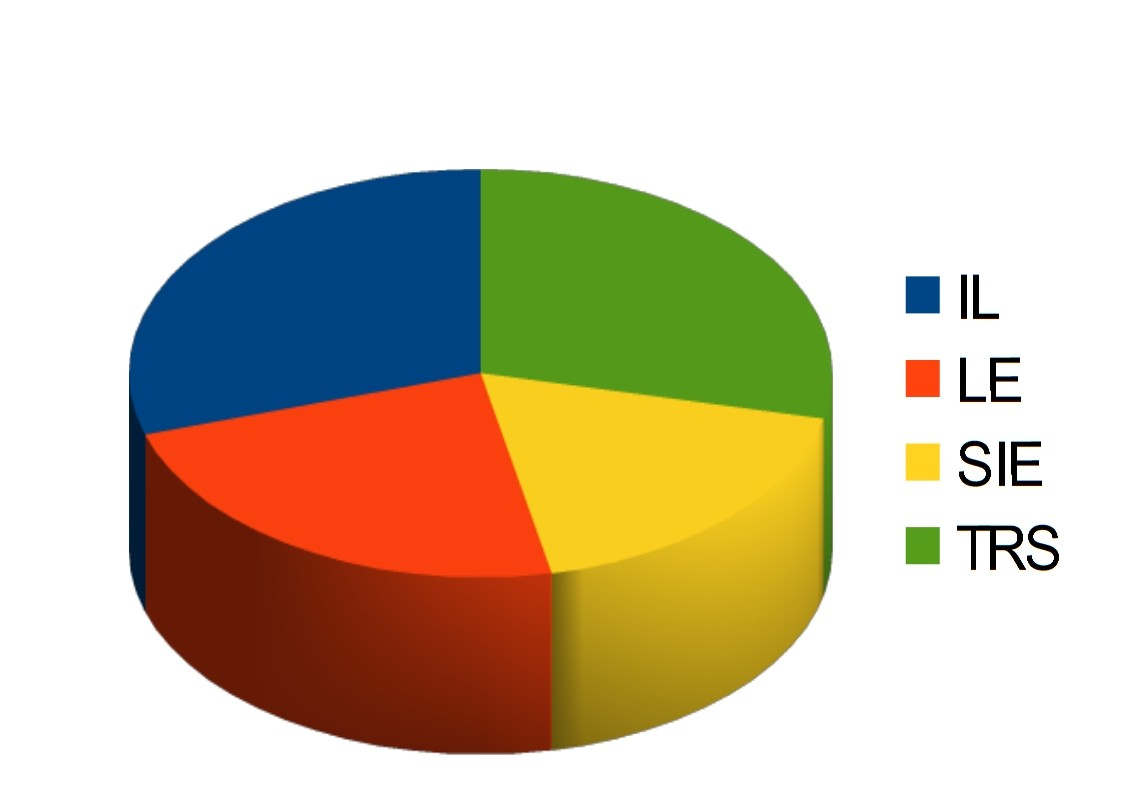
\includegraphics[width=100pt]{img/promo.jpg}
    \end{figure}
\end{frame}



\begin{frame}{Industrial project}
    Every part of a project represented\\
    \vfill
    A good occasion to discover the way to manage a project
    \vfill
    \begin{itemize}
	\item 4 students working for an enterprise
	\item 12 hours a week (about 250 hours per student)
	\item Use of a real project procedure
    \end{itemize}
\end{frame}


    
\begin{frame}{BH Consulting}
    Created by Bertrand PÉTAT in 2000.\\
    \vfill
    Human-scaled firm working in network implementation.\\
    \vfill
    Five employees:
    \begin{figure}
	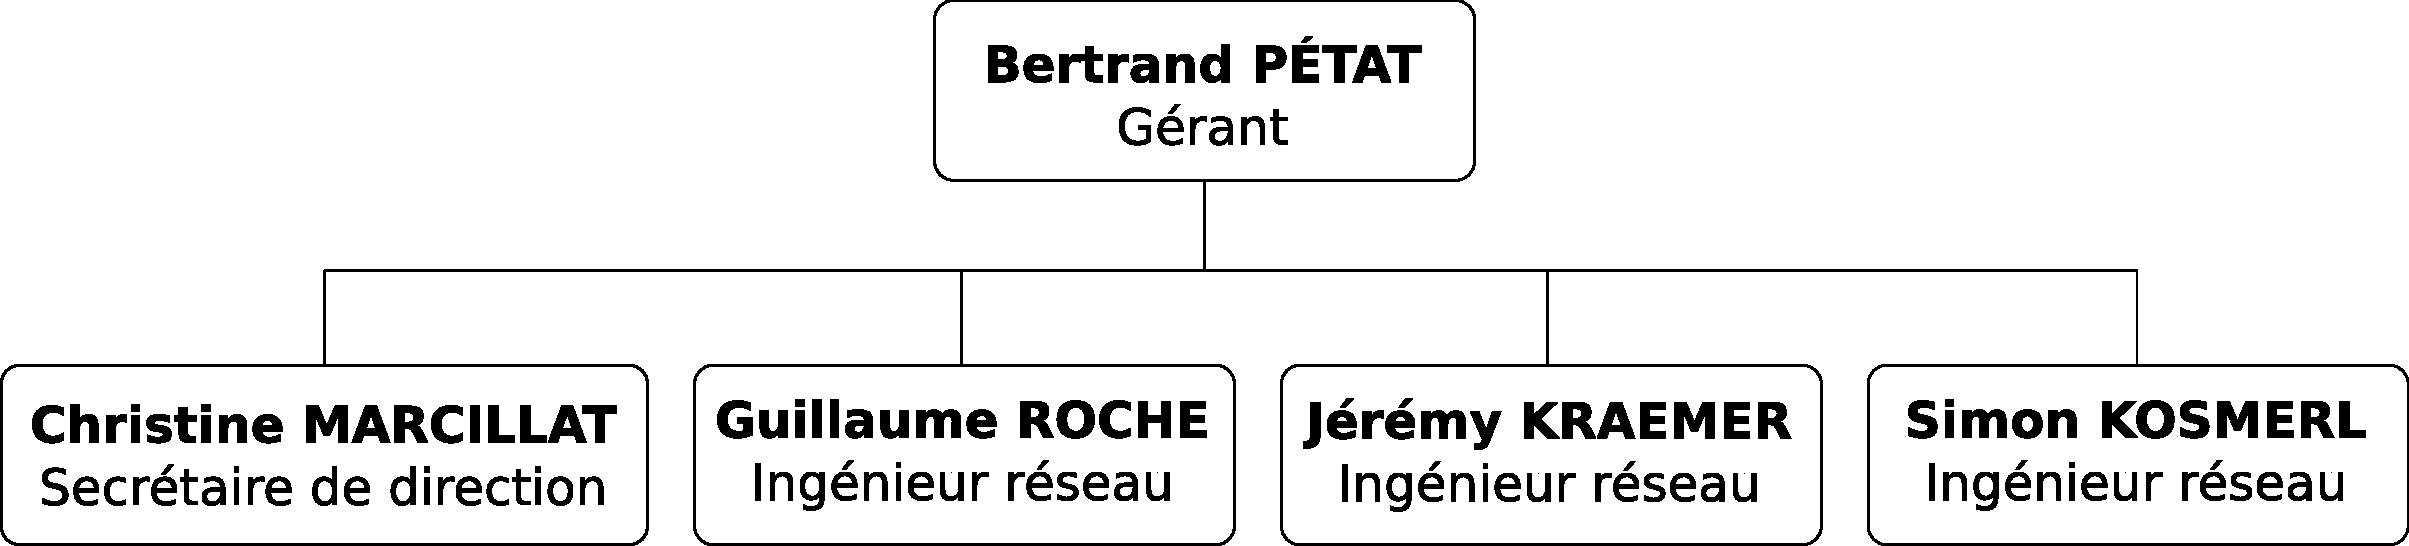
\includegraphics[width=300pt]{img/organigramme.pdf}
    \end{figure}
\end{frame}


\begin{frame}{Project motivations}
    \begin{itemize}
	\item<1->Network access control needed
	\vfill
	\item<2->Simplify access right management
	\vfill
	\item<3->Avoid repetitive tasks
    \end{itemize}

\end{frame}
    
\part{Organization}
\frame{\partpage}
\section{Organization}

\begin{frame}{Team presentation}
    \begin{itemize}
	\item {\bf Nicolas Bouget} \emph{TRS} Team leader \hfill 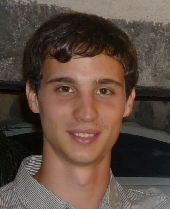
\includegraphics[width=30pt]{img/bouget.jpg}\\
	\vfill
	\item {\bf Julien Guepin} \emph{IL} Web developer \hfill 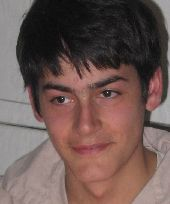
\includegraphics[width=30pt]{img/guepin.jpg}
	\vfill
	\item {\bf Marc Pinhede} \emph{LE} General developer\hfill 
\includegraphics[width=30pt]{img/pinhede.jpg}
	\vfill
	\item {\bf Julien Vaubourg} \emph{TRS} Network developer \hfill 
\includegraphics[width=30pt]{img/vaubourg.jpg}
    \end{itemize}
\end{frame}


\begin{frame}{VM Project}
    Software used to assist the team
    \vfill
    Assist the project manager to follow task progressions
    \vfill
    Gantt auto-generation
    \vfill
    Meeting report system
\end{frame}

\begin{frame}{Planning}
    %\includegraphics[widht=\paperwidht]{img/gant}
\end{frame}
    
\begin{frame}{Meeting}
    Meeting every monday with Guillaume Roche
    \vfill
    \begin{itemize}
	\item Week summary
	\item Questions 
	\item Directions 
    \end{itemize}
    \vfill
    More occasional meeting with our academic supervisor
\end{frame}


\part{Technical situation}
\frame{\partpage}
\section{Technical situation}

\begin{frame}{Client needs}
    \begin{itemize}
	\item Control network access for each client
	\vfill
	\item Monitor user sessions
	\vfill 
	\item Offer different ways of authentication
	\vfill
	\item Simplify network administration
	\vfill
	\item Keep traces of network configuration modifications
    \end{itemize}
\end{frame}

\begin{frame}{Implemented solution}
    Radius Server linked with MySql and 802.1X NAS
    \begin{itemize}
	\item<1-2> Network access controlled
	\item<2> Users accounting
    \end{itemize}
    \vfill
    Graphical web interface
    \begin{itemize}
	\item<0> Simplify user management
	\item<0> Permit easy authentication control
	\item<0> Offer an easy way to configure network
    \end{itemize}
    \vfill
    Version control system
\end{frame}
	
\begin{frame}{802.1X}
    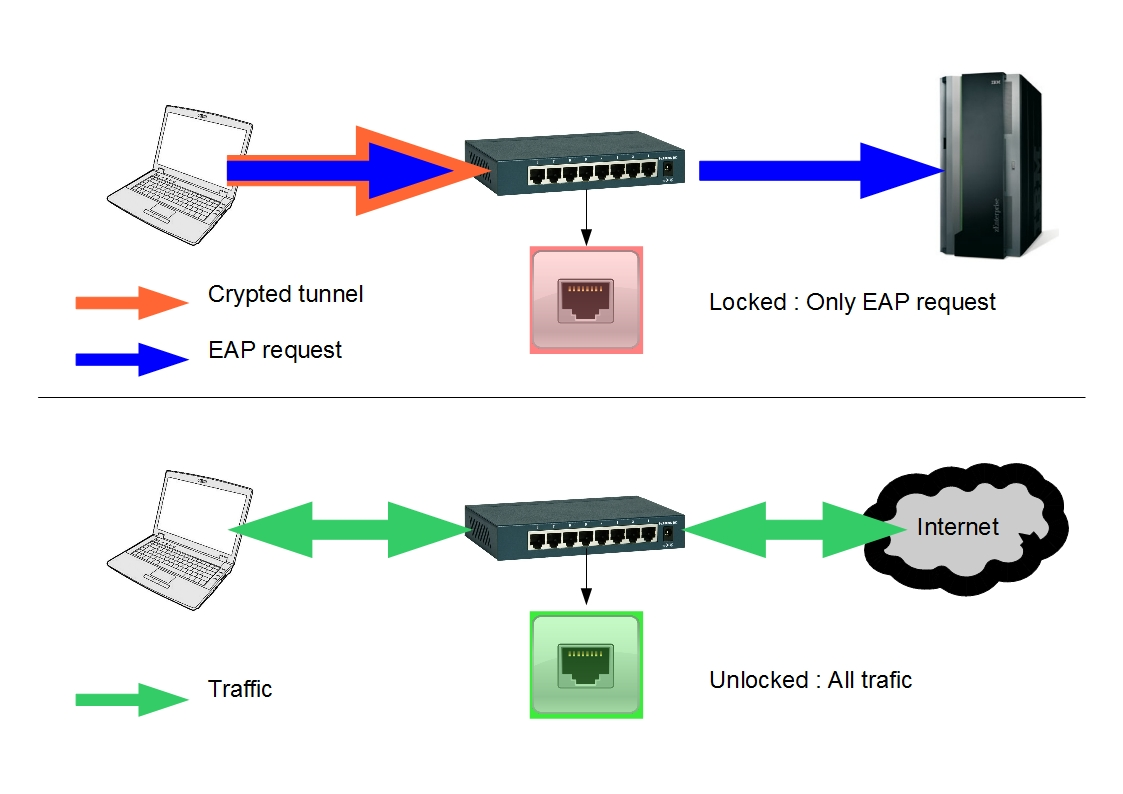
\includegraphics[width=300pts]{img/dot1x.jpg}
\end{frame}

\begin{frame}{Implemented solution}
    Radius Server linked with MySql and 802.1X NAS
    \begin{itemize}
	\item Network access controlled
	\item Users accounting
    \end{itemize}
    \vfill
    Graphical web interface
    \begin{itemize}
	\item<1-> Simplify user management
	\item<2-> Permit easy authentication control
	\item<3-> Offer an easy way to configure network
    \end{itemize}
    \vfill
    Version control system
\end{frame}

\begin{frame}{Current progression}
%grophique obtenable via bougboug?
\end{frame}


\begin{frame}{Conlusion}
    \begin{itemize}
	\item<1->Quick specification from BH Consulting
	\vfill
	\item<2->Some difficulties because of needed equipments
	\vfill
	\item<3->First part almost finished
	\vfill
	\item<4->Good investment of the team
    \end{itemize}
\end{frame}


\end{document}


